% arara: lualatex
% !TEX TS-program = LuaLaTeX


\documentclass{coderdojo}

\worksheet{8a}{Working with Lists I - Solutions}

\newcommand\contentsitem[2]{
	\item \hyperref[#1]{\color{section}\bfseries #2}
}

\usepackage{wrapfig}
\usepackage{float}

\newcommand\TODO[2][]{{\color{todo}
\gdef\ITEM{\item[\todoSymbol]}
\begin{itemize}
\ITEM {#1} #2
\end{itemize}}}

\newcommand\COMMENT[1]{{\color{comment}
\gdef\ITEM{\item[\commentSymbol]}
\begin{itemize}
\ITEM #1
\end{itemize}}}


\newcommand\TEST[1][\bf Test your code!]{
	\centerline{\tikz\node[starburst, fill=yellow, draw=red, line width=2pt,align=center] {#1};}
}

\newcommand\TESTSMALL[2][\bf Test your code!]{
{\tikz[scale=#2]\node[starburst, fill=yellow, draw=red, line width=2pt,align=center] {#1};}
}

\usetikzlibrary{decorations,
decorations.pathreplacing,decorations.pathmorphing}

\newenvironment{clist}
{\begin{list}{$\bullet$}{\setlength{\leftmargin}{6pt}}}
{\end{list}}

% postit
\tikzstyle{postit}=[fill=yellow!50,draw,thick,
decorate, drop shadow,
decoration={random steps,segment length=3pt,amplitude=1pt},
text width=4cm, font=\smaller]

\tikzstyle{postitnumber}=[inner sep=2pt,fill=yellow!50,draw,circle,font={\bf\smaller[3]}]

\newcommand\postit[2][]{\tikz\node[postit,#1] {#2};}

\newcommand\solution[3]{
\lstinputlisting[numbers=none,linewidth=5.5cm,breaklines=true,firstline=#1,lastline=#2]{#3}}

\begin{document}
\maketitle

\section*{Introduction}

\codeandoutput{title={\code{list_tasks_start.py}}}{1}{20}{code}{list_tasks.py}{
\ttfamily\smaller 
Generated data is\\

[63, 2, 27, 22, 73, 67, 89, 8, 42, 2]
}

\begin{itemize}
\item
All problems use the same dataset, which is generated by the code shown in \code{list_tasks_start.py}. Changing the random seed, we can get different, but repeatable datasets.  
\item
Since all solutions will start with the code in \code{list_tasks_start.py} those lines are not repeated in the solutions here to save space. But the code need to be in the solution scripts AS IS, and coders append their solution. 
\item The intention here is to develop the understanding of loops and conditionals, and the difference between indexes and the data values in lists. So while many questions have a builtin function answer \code{min}, \code{reverse} etc.  we are only interested in solutions that avoid their use.
\item Recap of Python Loops:
\begin{itemize}
\item Use \code{for d in data:}\\
To have a loop variable, \code{d}, that runs over the data values in the list \code{data}.
\item Use \code{for k in range(len(data)):}\\
To have a loop variable, \code{k}, that runs over the indexes needed to access all the data values in list \code{data}. Then \code{k} is the index, while \code{data[k]} is the data value at that index.
\item Use \code{for k,d in enumerate(data):}\\
To have two loop variables, \code{k} and \code{d}, that runs over the indexes and the data values in the list \code{data}.  So \code{k} and \code{d} satisfy property \code{data[k]==d}.
\end{itemize}

\item The first few are warm up exercises and should be very doable, but near the end they get very hairy.  But it depends on the coder --- for those that need help I get them to redo problems using each of the different for loop patterns above (if applicable).  This will be of benefit to them later.
\end{itemize}

\section*{Programming Tasks} 

Using the generated dataset:

\vspace{6pt}
\centerline{\tikz
\node[fill=yellow!10,drop shadow, rounded corners=6pt] (M)
	{\Large\bfseries [63, 2, 27, 22, 73, 67, 89, 8, 42, 2]
};}

%: list_tasks_1
\TODO[{\code{list_tasks_1}\\[6pt]}]
{Save your \code{list_tasks_start.py} as \code{list_tasks_1.py}
and add code to print out the data value at index 5.}

%\mbox{}\hfill\tikz\node[minimum width=5cm,fill=yellow!10,drop shadow,rounded corners] {67};

Full solution is 

\codeandoutput{title={\code{list_task_1.py}}}{1}{20}{code}{list_task_1.py}{
\solution{1}{3}{code/list_task_1.out}
}

But only displaying required solution by coder we have
\codeandoutput{title={\code{list_task_1.py}}}{10}{20}{code}{list_task_1.py}{
\solution{3}{3}{code/list_task_1.out}
}


%: list_tasks_2
\TODO[{\code{list_tasks_2}\\[6pt]}]
{Save your \code{list_tasks_start.py} as \code{list_tasks_2.py}
and add code to print out the data values, with one value per line --- you need a \code{for} loop.}

%\mbox{}\hfill\tikz\node[align=left,minimum width=5cm,fill=yellow!10,drop shadow,rounded corners]{63\\2\\27\\22\\73\\67\\89\\8\\42\\2};

\codeandoutput{title={\code{list_task_2.py}}}{10}{21}{code}{list_task_2.py}{
\solution{3}{12}{code/list_task_2.out}}


\COMMENT{While any of the three approaches given above work. The first is the python preferred due to being the simplest.  However, the second approach is the one needed for the next question.}

%: list_tasks_3
\TODO[{\code{list_tasks_3}\\[6pt]}]
{Save your \code{list_tasks_start.py} as \code{list_tasks_3.py}
and add code to print out the data values, with one value per line but in reverse order.}

%\mbox{}\hfill\tikz\node[align=left,minimum width=5cm,fill=yellow!10,drop shadow,rounded corners] {2\\42\\8\\89\\67\\73\\22\\27\\2\\63};

\COMMENT{The sequence of suggestions that I would give here are:
\begin{enumerate}
\item Output list elements is in current order using second alternative of question 1.
\item Replace \code{data[k]} with \code{k} to output the index instead of the data values. This will produce \code{0,1,2,...}.
\item What mathematical operation do I need to change \code{0,1,2,...} to \code{9,8,7,...}?
\\\mbox{}\hfill --- Replace \code{k} by \code{9-k} or even better  \code{len(data)-1-k}.
\item 
So now we have the index in reverse order how do we get the corresponding data values?
\\\mbox{}\hfill --- Wrap \code{len(data)-1-k} by  \code{data[len(data)-1-k]}.

\end{enumerate}}

\codeandoutput{title={\code{list_task_3.py}}}{10}{21}{code}{list_task_3.py}{
\solution{3}{12}{code/list_task_3.out}}

\COMMENT{Python list have method \code{reverse} or we could use features of the \code{range} function which will greatly simplify this task but we want solutions that avoid such shortcuts.}

%: list_tasks_4
\TODO[{\code{list_tasks_4}\\[6pt]}]
{Save your \code{list_tasks_start.py} as \code{list_tasks_4.py}
and add code to print out the maximum data value in the list.}

\mbox{}\hfill\tikz\node[align=left,minimum width=5cm,fill=yellow!10,drop shadow,rounded corners] 
{89};

\COMMENT{The sequence of suggestions that I would give here are:
\begin{enumerate}
\item 
First we should use the \code{for d in data} loop since we are just interested in data values not their index/positions.
\item 
Do a thought experiment where I am showing you a deck of cards --- one at a time -- how do you determine what is my max card?
\\\mbox{}\hfill --- keep a record of max value seen so far.

\item 
And since computers are (fast but) stupid we need to explicitly set the value of our "max so far" before we start our loop (i.e., start showing each individual card).
\item
We have a few choices for the initial value of \code{myMax}. Setting it equal to the first element in the list is simplest (and we will do this here) but this can cause problems. Why?
\\\mbox{}\hfill --- what happens if the list is empty?
\end{enumerate}}

\codeandoutput{title={\code{list_task_4.py}}}{10}{21}{code}{list_task_4.py}{
\solution{3}{12}{code/list_task_4.out}}

%: list_tasks_5
\TODO[{\code{list_tasks_5}\\[6pt]}]
{Save your \code{list_tasks_start.py} as \code{list_tasks_5.py}
and add code to print out the minimum data value in the list.}

\mbox{}\hfill\tikz\node[align=left,minimum width=5cm,fill=yellow!10,drop shadow,rounded corners] 
{2};

\COMMENT{
\begin{enumerate}
\item
This problem is here to make sure that coders understood the previous task. The only difference here is keeping a record of the smallest value seen so far instead of the largest value.
\item 
Make sure good variable names are used \code{myMin} not \code{myMax}
\end{enumerate}}

\codeandoutput{title={\code{list_task_5.py}}}{10}{21}{code}{list_task_5.py}{
\solution{3}{12}{code/list_task_5.out}}


%: list_tasks_6
\TODO[{\code{list_tasks_6}\\[6pt]}] 
{Save your \code{list_tasks_start.py} as \code{list_tasks_6.py}
and add code to print out the difference between the maximum value and the minimum data value in 
the list.}

\COMMENT{
\begin{enumerate}
\item
Start by getting the code for keeping track of the max and the min seen so far working.
\item 
Should do this in a single foo loop.
\item 
Use \code{print(myMax,myMin)} to output both values to help debugging.
\item 
Finally edit print function to output difference.
\end{enumerate}}

\mbox{}\hfill\tikz\node[align=left,minimum width=5cm,fill=yellow!10,drop shadow,rounded corners] 
{87};

\codeandoutput{title={\code{list_task_6.py}}}{10}{21}{code}{list_task_6.py}{
\solution{3}{12}{code/list_task_6.out}}

%: list_tasks_7
\TODO[{\code{list_tasks_7}\\[6pt]}] 
{Save your \code{list_tasks_start.py} as \code{list_tasks_7.py}
and add code to print out the index of the maximum value in the list. 
\\If the maximum value appears more than once, then print out index of first occurrence. 
}

\mbox{}\hfill\tikz\node[align=left,minimum width=5cm,fill=yellow!10,drop shadow,rounded corners] 
{6};

\COMMENT{
\begin{enumerate}
\item
Now these tasks are beginning to get a little harder. Here we want both data values (to see what is the max value) and indexes/positions (to see where the max value is).  So use the third loop alternative given in task 1.
\item
Using the \code{for k,d in enumerate(data)} loop we find the max value as usual.
\item
Next we add code to keep a record of the index as well, don't forget to initialise this variable before the loop.
\end{enumerate}}

\codeandoutput{title={\code{list_task_7.py}}}{10}{21}{code}{list_task_7.py}{
\solution{3}{12}{code/list_task_7.out}}

\vfill

%: list_tasks_8
\TODO[{\code{list_tasks_8}\\[6pt]}] 
{Save your \code{list_tasks_start.py} as \code{list_tasks_8.py}
and add code to print out the index of the minimum value in the list. 
\\If the minimum value appears more than once, then print out index of first occurrence. 
}

\mbox{}\hfill\tikz\node[align=left,minimum width=5cm,fill=yellow!10,drop shadow,rounded corners] 
{0};

\COMMENT{
\begin{enumerate}
\item Like tasks 4 and 5, this is very similar to task 7 to check understanding.
% But here there is a small wrinkle --- if the index is not initialised before the for loop the output will be incorrect. 
\item You could ask how to modify solution so that it outputs position of last min value.
\end{enumerate}}

\codeandoutput{title={\code{list_task_8.py}}}{10}{31}{code}{list_task_8.py}{
\solution{3}{3}{code/list_task_8.out}}

\vfill\mbox{}

\newpage

%: list_tasks_9
\TODO[{\code{list_tasks_9}\\[6pt]}] 
{Save your \code{list_tasks_start.py} as \code{list_tasks_9.py}
and add code to print out the total of the data values in the list.
}

\mbox{}\hfill\tikz\node[align=left,minimum width=5cm,fill=yellow!10,drop shadow,rounded corners] 
{395};

\COMMENT{
\begin{enumerate}
\item
Since we only need the data values, we can go back to using the easier \code{for d in data} type loop.
\item
We need to keep a running total of the data values seen so far.
\end{enumerate}}


\codeandoutput{title={\code{list_task_9.py}}}{10}{21}{code}{list_task_9.py}{
\solution{3}{12}{code/list_task_9.out}}

\vfill 
%: list_tasks_10
\TODO[{\code{list_tasks_10}\\[6pt]}] 
{Save your \code{list_tasks_start.py} as \code{list_tasks_10.py}
and add code to print out the total of all of the even data values minus the total of the odd data values in the list.
}

\mbox{}\hfill\tikz\node[align=left,minimum width=5cm,fill=yellow!10,drop shadow,rounded corners] 
{-243};

\COMMENT{
\begin{enumerate}
\item
First modify the previous solution so that the total only involves the even numbers. To check if data value \code{d} is even we use \code{d\%2==0}.
\item
Next modify to have update a second total, the total of odd numbers.
\item
Finally print out the difference.
\item 
Note that there is a solution using only one total and does addition/subtraction within the loop.
\end{enumerate}}

\codeandoutput{title={\code{list_task_10.py}}}{10}{31}{code}{list_task_10.py}{
\solution{3}{3}{code/list_task_10.out}}

\newpage

%: list_tasks_11
\TODO[{\code{list_tasks_11}\\[6pt]}]  
{Save your \code{list_tasks_start.py} as \code{list_tasks_11.py}
and add code to print out the second largeest data value in the list.}

\mbox{}\hfill\tikz\node[align=left,minimum width=5cm,fill=yellow!10,drop shadow,rounded corners] 
{73};

\COMMENT{
\begin{enumerate}
\item
We need to keep track of two data values --- the largest found so far and the second largest found so far.
\item
We update the second largest when we get a data value (\code{d}) larger than the second largest found so far (\code{mySecondMax}) but less than the max found so far (\code{myMax}).

\begin{center}
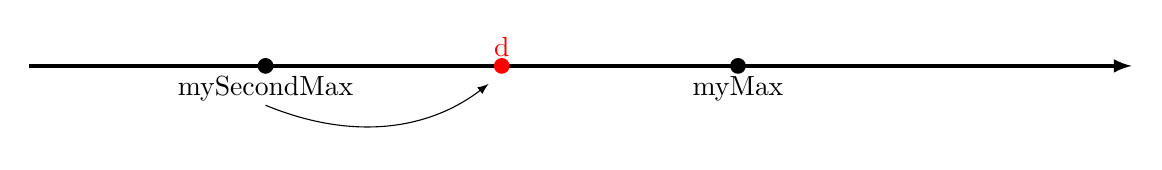
\begin{tikzpicture}
	\draw[-latex,very thick] (0,0)  
	-- node[below]{\code{mySecondMax}} ++(6,0)
	-- node[below]{\code{myMax}} ++(6,0) -- ++(2,0);
	\fill (3,0) circle (.1);
	\fill (9,0) circle (.1);
	\fill[red] (6,0) circle (.1) node[above] {\code{d}};
	\draw[-latex,shorten >=6pt] (3,-.5) to[bend right] (6,-0.1);
\end{tikzpicture}
\end{center}
\item
We update both the second largest and the largest when we get a value that is larger than the max found so far.

\begin{center}
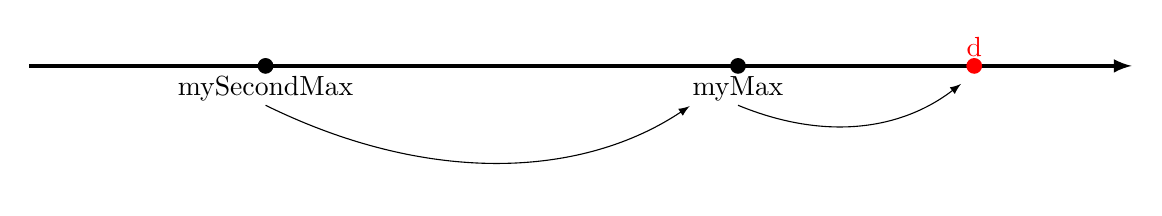
\begin{tikzpicture}
	\draw[-latex,very thick] (0,0)  
	-- node[below]{\code{mySecondMax}} ++(6,0)
	-- node[below]{\code{myMax}} ++(6,0) -- ++(2,0);
	\fill (3,0) circle (.1);
	\fill (9,0) circle (.1);
	\fill[red] (12,0) circle (.1) node[above] {\code{d}};
	\draw[-latex,shorten >=21pt] (3,-.5) to[bend right] (9,-0.1);
	\draw[-latex,shorten >=6pt] (9,-.5) to[bend right] (12,-0.1);
\end{tikzpicture}
\end{center}
\end{enumerate}}

\codeandoutput{title={\code{list_task_11.py}}}{10}{21}{code}{list_task_11.py}{
\solution{3}{12}{code/list_task_11.out}}

\end{document}

